%% ============================================================
%%  HLT diphoton trigger efficiency 2024 -- new eta-R9 map
%%  Beamer / pdflatex. Style copied from
%%    /home/santanu/Documents/2023_lowmass_analysis/src/india_cms_2026.tex
%%  Every number on these slides is printed by
%%    ../notebooks/02_map_and_efficiency_study.ipynb  (section [M] -> ../data/slide_numbers.json)
%%  or read from ../data/counting_vs_fit.csv / ../data/efficiency_three_way.csv.
%% ============================================================
\documentclass[aspectratio=169,10pt]{beamer}

\usepackage[T1]{fontenc}
\usepackage[utf8]{inputenc}
\usepackage{lmodern}
\usepackage{graphicx}
\usepackage{booktabs}
\usepackage{array}
\usepackage{xcolor}
\usepackage{amsmath}
\usepackage{amssymb}
\usepackage{microtype}
\usepackage{hyperref}
\usepackage{appendixnumberbeamer}
\usepackage{tikz}

\graphicspath{{../plots/}}

% ── Colour palette (CMS dark-navy style) ─────────────────────
\definecolor{navydark}  {RGB}{10,  27, 56}
\definecolor{navymid}   {RGB}{18,  48, 96}
\definecolor{cmsblue}   {RGB}{ 0, 112,192}
\definecolor{cmsaccent} {RGB}{ 0, 188,235}
\definecolor{cmsgold}   {RGB}{255,185,  0}
\definecolor{lightgrey} {RGB}{210,220,235}
\definecolor{offwhite}  {RGB}{240,244,250}
\definecolor{cmsgreen}  {RGB}{  0,190,120}

\usetheme{default}
\setbeamertemplate{navigation symbols}{}
\setbeamertemplate{itemize item}{\color{cmsaccent}\small$\blacktriangleright$}
\setbeamertemplate{itemize subitem}{\color{cmsgold}\footnotesize$\bullet$}
\setbeamercolor{background canvas}{bg=navydark}
\setbeamercolor{normal text}{fg=offwhite}
\setbeamercolor{alerted text}{fg=cmsgold}
\setbeamercolor{frametitle}{fg=cmsaccent, bg=navymid}
\setbeamerfont{frametitle}{size=\large, series=\bfseries}
\setbeamertemplate{frametitle}{%
  \vskip2pt
  \hspace*{6pt}\insertframetitle
  \vskip3pt
  \color{cmsaccent}\rule{\linewidth}{0.4pt}%
  \vskip2pt
}
\setbeamercolor{structure}{fg=cmsaccent}
\setbeamercolor{footline}{fg=lightgrey, bg=navymid}
\setbeamertemplate{footline}{%
  \begin{beamercolorbox}[wd=\paperwidth,ht=2.2ex,dp=1ex]{footline}
    \hspace*{6pt}\tiny HLT efficiency 2024 --- new $\eta$--$R_9$ map
    \hfill \tiny\insertframenumber\,/\,\inserttotalframenumber\hspace*{6pt}
  \end{beamercolorbox}%
}
\hypersetup{colorlinks=true, urlcolor=cmsaccent, linkcolor=cmsaccent}

\newcommand{\pT}{\ensuremath{p_{\mathrm{T}}}}
\newcommand{\ET}{\ensuremath{E_{\mathrm{T}}}}
\newcommand{\RNine}{\ensuremath{R_{9}}}
\newcommand{\hl}[1]{\textcolor{cmsaccent}{\textbf{#1}}}
\newcommand{\gold}[1]{\textcolor{cmsgold}{\textbf{#1}}}
\newcommand{\plotslide}[3][0.80]{%
  \begin{center}
    \colorbox{white}{\includegraphics[width=#1\linewidth,height=0.70\textheight,keepaspectratio]{#2}}\\[2pt]
    {\tiny\color{lightgrey}#3}
  \end{center}}
\newcommand{\wimg}[2]{\colorbox{white}{\includegraphics[width=#1,height=0.68\textheight,keepaspectratio]{#2}}}
\newcommand{\partdivider}[2]{%
  {\setbeamercolor{background canvas}{bg=navymid}
   \setbeamertemplate{footline}{}
   \begin{frame}[plain,noframenumbering]
     \vspace*{2.0cm}\centering
     {\large\color{lightgrey} #1}\\[8pt]
     {\huge\bfseries\color{cmsaccent} #2}
   \end{frame}}}
\newcommand{\cmprow}[3]{% set, leg, region: three or two category plots
  \begin{columns}[T,onlytextwidth]#3\end{columns}}

\begin{document}

% ── Title ────────────────────────────────────────────────────
{\setbeamertemplate{footline}{}
\setbeamercolor{background canvas}{bg=white}
\setbeamercolor{normal text}{fg=navymid}
\begin{frame}[plain]
  \vspace*{1.4cm}\centering
  {\color{cmsaccent}\rule{0.6\linewidth}{1.5pt}}\\[14pt]
  {\Large\bfseries\color{navymid} HLT diphoton efficiency 2024}\\[6pt]
  {\Large\bfseries\color{navymid} with the new $\eta$--$R_9$ reweighting map}\\[12pt]
  {\color{cmsaccent}\rule{0.6\linewidth}{1.5pt}}\\[24pt]
  {\large\color{navymid} Santanu Mahata \quad Rajdeep Chatterjee}\\[6pt]
  {\footnotesize\color{navymid} Tata Institute of Fundamental Research}
  \vfill
  \noindent\hfill
  
\includegraphics[width=1.75cm]{tifr_logo_white_background.png}\hspace{8pt}
  
\includegraphics[height=0.95cm]{cms_logo.png}
\end{frame}}

% ── What is compared ─────────────────────────────────────────
\begin{frame}{What is compared}
  \centering
  {\scriptsize
  \begin{tabular}{@{}p{0.15\linewidth}p{0.36\linewidth}p{0.45\linewidth}@{}}
    \toprule
    \textbf{Set} & \textbf{Source} & \textbf{$\eta$--\RNine{} weight} \\
    \midrule
    \textcolor{cmsgreen}{\textbf{2023 (postBPix)}} & HLT-diphoton-efficiency-2023-results @ \texttt{9450e11} & as used for 2023 \\
    \textcolor{cmsaccent}{\textbf{2024 repo}} & HLT-diphoton-efficiency-2024-results @ \texttt{d422813}, \texttt{etaR9rw\_withPresel} & old map: \texttt{2024\_R9\_vs\_eta\_HggOverDY\_presel\_vf.root} \\
    \textcolor{red!70!white}{\textbf{2024 local}} & fits run 2026-10-01/02 on lxplus & new map: \texttt{2024Lowmass\_R9\_vs\_eta\_ratio\_presel.root} \\
    \bottomrule
  \end{tabular}}
  \vspace{6pt}
  \begin{itemize}\footnotesize
    \item \gold{2024 repo vs 2024 local:} input trees differ only in \texttt{r9etaWeight\_with\_presel} and \texttt{weight\_with\_presel};
          all 76 branches of all 159\,861\,517 entries per leg read back and compared.
    \item Same 20 settings files and the same \texttt{run\_HLT\_2024\_all.sh} (byte-identical local copies).
    \item Both maps: $25\times16$ cells in (full5x5 \RNine, $|\eta|$), identical bin edges.
    \item Nominal fit everywhere: BW$\otimes$DSCB signal + RooCMSShape background.
    \item \gold{Errors: stat $\oplus$ syst} --- fit error $\oplus$ $|\varepsilon_{\rm CMSShape}-\varepsilon_{\rm Exp}|$, upper error capped at $1-\varepsilon$:
          the \texttt{total\_unc} definition of the 2023 CSV (reproduced to $10^{-4}$), applied to both 2024 sets.
  \end{itemize}
  \vfill
  {\tiny\color{lightgrey} Not verified: the settings and trees that sat on lxplus for the August repo run (local copies only); fitter source between August and October.}
\end{frame}

% ── Preselection and binning (as india_cms_2026) ─────────────
\begin{frame}{Offline photon preselection for 2024 (same as 2023), and the binning}
  \centering
  {\footnotesize
  \begin{tabular}{@{}lccccc@{}}
    \toprule
    \textbf{Category} & $H/E$ & $\sigma_{i\eta i\eta}$ & \RNine{} & \texttt{Rho\_PfPhoISO03} & \texttt{TrackerISO03} \\
    \midrule
    Barrel, $\RNine < 0.85$ & $< 0.08$ & $< 0.011$ & $> 0.5$ & $< 3.0$ & $< 6.0$ \\
    Barrel, $\RNine > 0.85$ & $< 0.08$ & $< 0.011$ & $> 0.5$ & $< 3.0$ & $< 6.0$ \\
    Endcap, $\RNine > 0.9$  & $< 0.08$ & $< 0.032$ & $> 0.9$ & $< 3.0$ & $< 6.0$ \\
    \bottomrule
  \end{tabular}}

  \vspace{7pt}
  {\footnotesize
  \begin{tabular}{@{}lcl@{}}
    \toprule
    \textbf{Leg} & \textbf{Bins} & \textbf{Probe $E_{T}$ bin edges [GeV]} \\
    \midrule
    seeded (30~GeV)   & 9  & 0, 35, 37, 40, 45, 50, 60, 70, 90, $\infty$ \\
    unseeded (18~GeV) & 12 & 0, 21, 25, 28, 31, 35, 40, 45, 50, 60, 70, 90, $\infty$ \\
    \midrule
    \multicolumn{3}{@{}l@{}}{\textbf{5 \RNine{}/$\eta$ categories on each leg:}\;
      EB $0.50$--$0.55$, EB $0.55$--$0.85$, EB $>0.85$, EE $0.90$--$0.93$, EE $>0.93$} \\
    \bottomrule
  \end{tabular}}
  \vspace{4pt}

  {\scriptsize 105 fitted \ET{} points per set; efficiency plots do not draw the catch-all first bin (0--35 / 0--21~GeV) and draw the last bin as 90--110~GeV.}
\end{frame}

% ── Efficiency comparison, normal set ───────────────────────
\begin{frame}{2023 vs 2024 repo vs 2024 local --- seeded leg, EB bins}
  \begin{columns}[T,onlytextwidth]
    \column{0.33\textwidth}\centering\wimg{\linewidth}{eff/eff_normal_seed_EB_R9_0p50to0p55.pdf}
    \column{0.33\textwidth}\centering\wimg{\linewidth}{eff/eff_normal_seed_EB_R9_0p55to0p85.pdf}
    \column{0.33\textwidth}\centering\wimg{\linewidth}{eff/eff_normal_seed_EB_R9gt0p85.pdf}
  \end{columns}
  \vspace{2pt}
  {\tiny\color{lightgrey} Error bars: stat $\oplus$ syst. Lower pad: ratio to 2024 repo, the two uncertainties added in quadrature.}
\end{frame}

\begin{frame}{2023 vs 2024 repo vs 2024 local --- seeded leg, EE bins}
  \begin{columns}[T,onlytextwidth]
    \column{0.44\textwidth}\centering\wimg{\linewidth}{eff/eff_normal_seed_EE_R9_0p90to0p93.pdf}
    \column{0.44\textwidth}\centering\wimg{\linewidth}{eff/eff_normal_seed_EE_R9gt0p93.pdf}
  \end{columns}
  \vspace{2pt}
  {\tiny\color{lightgrey} Error bars: stat $\oplus$ syst. Lower pad: ratio to 2024 repo, the two uncertainties added in quadrature.}
\end{frame}

\begin{frame}{2023 vs 2024 repo vs 2024 local --- unseeded leg, EB bins}
  \begin{columns}[T,onlytextwidth]
    \column{0.33\textwidth}\centering\wimg{\linewidth}{eff/eff_normal_unseed_EB_R9_0p50to0p55.pdf}
    \column{0.33\textwidth}\centering\wimg{\linewidth}{eff/eff_normal_unseed_EB_R9_0p55to0p85.pdf}
    \column{0.33\textwidth}\centering\wimg{\linewidth}{eff/eff_normal_unseed_EB_R9gt0p85.pdf}
  \end{columns}
  \vspace{2pt}
  {\tiny\color{lightgrey} Error bars: stat $\oplus$ syst. Lower pad: ratio to 2024 repo, the two uncertainties added in quadrature.}
\end{frame}

\begin{frame}{2023 vs 2024 repo vs 2024 local --- unseeded leg, EE bins}
  \begin{columns}[T,onlytextwidth]
    \column{0.44\textwidth}\centering\wimg{\linewidth}{eff/eff_normal_unseed_EE_R9_0p90to0p93.pdf}
    \column{0.44\textwidth}\centering\wimg{\linewidth}{eff/eff_normal_unseed_EE_R9gt0p93.pdf}
  \end{columns}
  \vspace{2pt}
  {\tiny\color{lightgrey} Error bars: stat $\oplus$ syst. Lower pad: ratio to 2024 repo, the two uncertainties added in quadrature.}
\end{frame}

\begin{frame}{Where the 2024 efficiency moved: local $-$ repo, every bin}
  \plotslide[0.95]{diff/heat_local_minus_repo_normal.pdf}
    {Top: absolute difference. Bottom: difference / ($\sigma_{\rm repo}\oplus\sigma_{\rm local}$), $\sigma$ = stat $\oplus$ syst; both fits use the same events, so this treats correlated numbers as independent.}
  \vspace{-6pt}
  {\scriptsize Mean $|\Delta|$ = 0.0048 over 105 bins. 10 bins with $|\Delta|>0.01$: 9 unseeded, 8 of them with $\ET<31$~GeV. Largest $|\Delta|/\sigma$: 1.65.}
\end{frame}

% ── Part: the maps ───────────────────────────────────────────
\partdivider{Part II}{The two $\eta$--$R_9$ maps}

\begin{frame}{Old map vs new map}
  \begin{columns}[T,onlytextwidth]
    \column{0.5\textwidth}\centering\wimg{\linewidth}{maps/map_old_map_2024_repo.pdf}
    \column{0.5\textwidth}\centering\wimg{\linewidth}{maps/map_new_map_2024_local.pdf}
  \end{columns}
  \vspace{4pt}
  \begin{itemize}\scriptsize
    \item Old: Hgg / DY MC, density-normalised, empty-DY cell $\to$ 1 (\texttt{.meta} file). Range 0.42--5.29; 118 cells exactly 1.
    \item New: no metadata file; recorded as ``used as supplied'' at weight replacement; user describes it as normalising-flow based. Range 0--5.93; 4 cells exactly 0.
  \end{itemize}
\end{frame}

\begin{frame}{New $-$ old, cell by cell}
  \plotslide[0.92]{maps/map_new_old.pdf}
    {Drawn in bin-index space (\RNine{} bins are 0.5, 0.05, 0.02 and 0.01 wide); dashed lines bound the EB--EE gap row. new/old ranges 0 to 4.62 (\texttt{maps/map\_new\_old.pdf} has the ratio).}
\end{frame}

\begin{frame}{Map slices: weight vs \RNine{} in every $|\eta|$ row}
  \plotslide[0.80]{maps/map_slices_vs_r9.pdf}
    {Shaded: the \RNine{} windows of the analysis categories in EB and EE rows.}
\end{frame}

\begin{frame}{Which cells the probes actually use}
  \centering
  \wimg{0.98\linewidth}{why/occupancy_seed.pdf}\\[2pt]
  \wimg{0.98\linewidth}{why/occupancy_unseed.pdf}\\[2pt]
  {\tiny\color{lightgrey} Selected probes per map cell (normal set, pass+fail, $60<m<120$~GeV), top seeded, bottom unseeded. Hatched: old map $=1$ (\texttt{//}), new map $=0$ (\texttt{xx}). Selected probes in either kind of cell: 0 in every category.}
\end{frame}

\begin{frame}{Per-probe weights and effective statistics}
  \plotslide[0.95]{why/weights_and_neff.pdf}
    {Left: per-probe weight distribution of all selected probes. Right: effective number of failing probes $N_{\rm eff}=(\sum w)^2/\sum w^2$, new / old map, per bin: 0.92--1.01.}
\end{frame}

% ── Part: why ────────────────────────────────────────────────
\partdivider{Part III}{Do the weights explain the shifts?}

\begin{frame}{Method: what the weights alone do}
  \begin{itemize}\footnotesize
    \item Both weights are a pure lookup in the map: every selected probe's stored weight equals its cell value
          (0 mismatches in 2$\times$159.9\,M entries, old and new).
    \item So, per fitter bin, count probes per map cell once, separately for pass and fail. Any map then gives
          \[ P=\sum_c N^{\rm pass}_c\,w_c,\qquad F=\sum_c N^{\rm fail}_c\,w_c,\qquad
             \varepsilon_{\rm count}=\frac{P}{P+F}. \]
    \item Cuts, flags and \ET{} bins parsed from the 20 settings files; $60<m<120$~GeV.
          Rebuilt yields equal the sums of stored weights to $1.4\times10^{-8}$ (relative).
    \item $\varepsilon_{\rm count}$ includes background --- it is \hl{not} the fitted efficiency.
          $\Delta\varepsilon_{\rm count}=\varepsilon^{\rm new}_{\rm count}-\varepsilon^{\rm old}_{\rm count}$ is the change from the map alone, with no fit.
  \end{itemize}
\end{frame}

\begin{frame}{Fitted shift vs shift from the weights alone --- unseeded}
  \plotslide[0.98]{why/fit_vs_count_vs_pt_normal_unseed.pdf}
    {Red: fitted local $-$ repo. Black: $\Delta\varepsilon_{\rm count}$. Grey: $\pm(\sigma_{\rm repo}\oplus\sigma_{\rm local})$, stat $\oplus$ syst.}
  \vspace{-4pt}
  {\scriptsize Largest $|\Delta\varepsilon_{\rm count}|$ in any bin: 0.0048 (normal), 0.0043 (fullPath). Largest fitted $|\Delta|$: 0.114.}
\end{frame}

\begin{frame}{Every bin: fitted shift vs counting shift; normal vs fullPath}
  \begin{columns}[T,onlytextwidth]
    \column{0.38\textwidth}\centering\wimg{\linewidth}{why/fit_vs_count_scatter_normal.pdf}
    \column{0.62\textwidth}\centering\wimg{\linewidth}{why/normal_vs_fullPath_shifts.pdf}
  \end{columns}
  \vspace{2pt}
  {\scriptsize Correlation of fitted and counting shift: 0.18 (normal), 0.56 (fullPath).
   Same map, extra \texttt{probe\_passFullPath==1}: largest fitted $|\Delta|$ 0.114 (normal) vs 0.0083 (fullPath).}
\end{frame}

\begin{frame}{The six largest fitted shifts, cell by cell}
  \plotslide[0.92]{why/cell_decomposition_top6.pdf}
    {First-order contribution of each cell to $\Delta\varepsilon_{\rm count}$; $\Sigma$ cells vs exact counting shift in each title.}
  \vspace{-6pt}
  {\scriptsize In 4 of the 6, $\Delta\varepsilon_{\rm count}$ has the opposite sign to the fitted shift; in all 6, $|\Delta\varepsilon_{\rm count}|\le0.0048$.}
\end{frame}

\begin{frame}{Mean weight of passing vs failing probes --- unseeded}
  \plotslide[0.98]{why/wpass_over_wfail_unseed.pdf}
    {$\varepsilon_{\rm count}$ changes only through $\langle w\rangle_{\rm pass}/\langle w\rangle_{\rm fail}$; shown for both maps.}
\end{frame}

\begin{frame}{The largest shift in the fit: unseeded EE $\RNine>0.93$, $\ET<21$~GeV}
  \centering
  \colorbox{white}{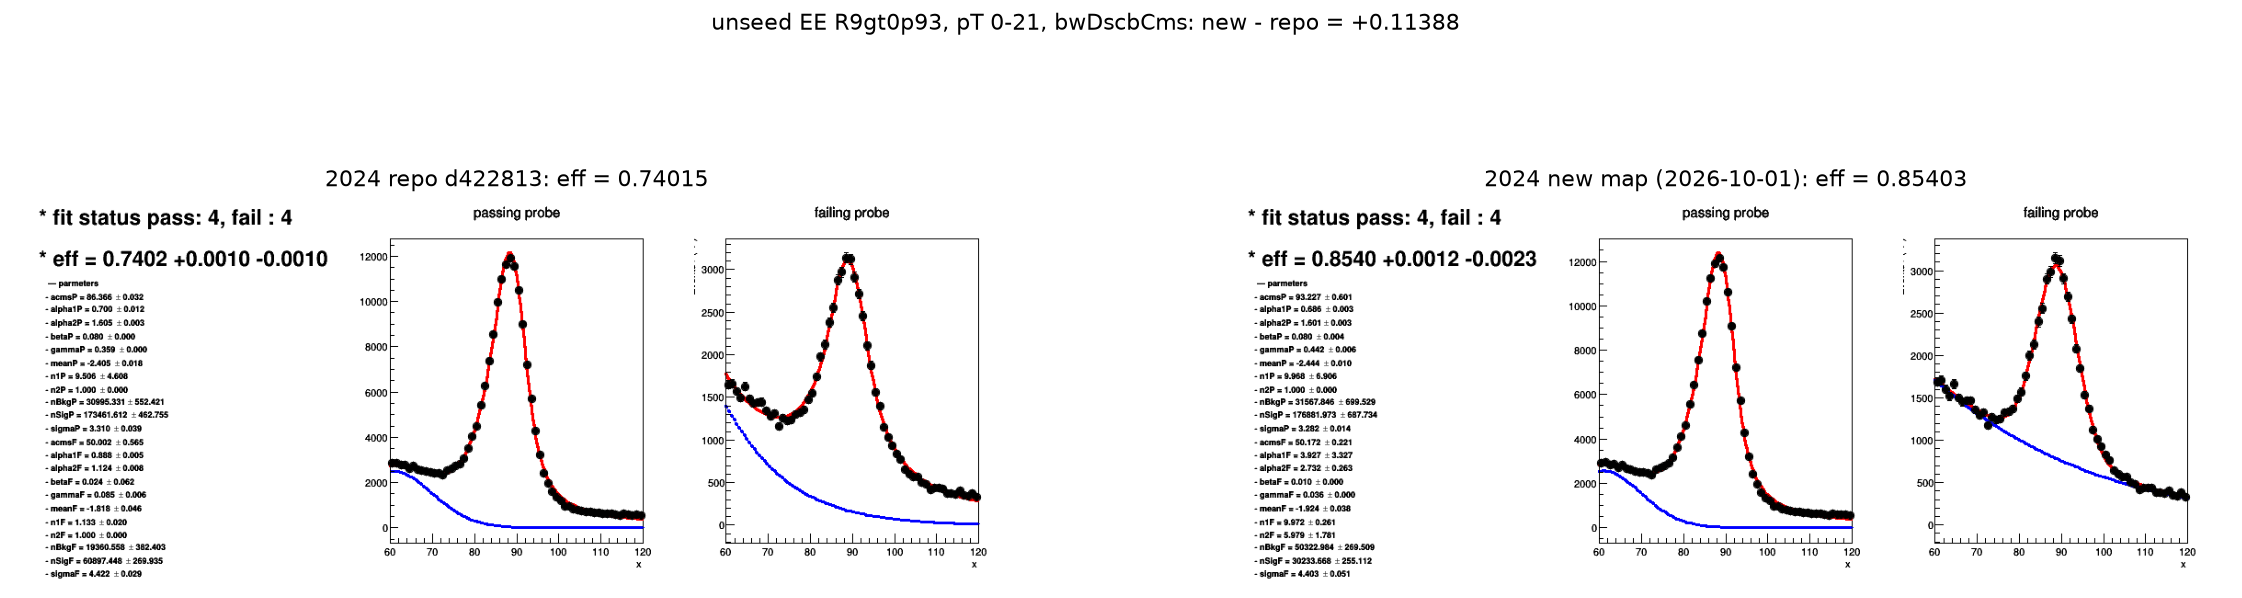
\includegraphics[width=0.98\linewidth,height=0.55\textheight,keepaspectratio]{why/fit_shift1_unseed_EE_R9gt0p93_0_bwDscbCms.png}}\\[3pt]
  {\scriptsize Left repo (old map), right local (new map). Both print \texttt{fit status pass: 4, fail: 4}.
   Failing-probe fit: background yield 19\,361 $\to$ 50\,323, signal yield 60\,897 $\to$ 30\,234 (values printed on the plots).
   Counting shift for this bin: $+0.0030$; fitted shift $+0.114$.}
\end{frame}

\begin{frame}{Summary}
  \begin{itemize}\footnotesize
    \item \gold{Efficiencies.} Normal set: mean $|$local$-$repo$|$ = 0.0048; 10 of 105 bins move by more than 0.01, 9 unseeded, 8 below 31~GeV; max 0.114.
          fullPath: max 0.0083, none above 0.01. With stat $\oplus$ syst errors, largest $|\Delta|/\sigma$: 1.65 (normal), 2.05 (fullPath).
    \item \gold{Largest bin} (unseeded EE $\RNine>0.93$, $<21$~GeV): local CMSShape and Exp fits disagree by 0.098, so its syst dominates its error.
    \item \gold{Maps.} Same binning; new/old from 0 to 4.62. The old map's 118 cells at 1 and the new map's 4 zero cells hold no selected probes.
    \item \gold{Weights alone.} Map change moves $\varepsilon_{\rm count}$ by at most 0.0048 in any bin; effective failing-probe statistics change by $-8\%$ to $+0.5\%$.
    \item \gold{So:} the large fitted shifts in low-\ET{} unseeded bins are not reproduced by the weights alone,
          and are absent in fullPath with the same weights. The one fit pair inspected shows the failing-probe signal/background split changing.
    \item \gold{Next (proposal):} check fit stability of those bins (fit status 4, starting values, background model) before using either set.
  \end{itemize}
  \vfill
  {\tiny\color{lightgrey} Code and numbers: \texttt{notebooks/01\_scan\_trees\_per\_map\_cell.ipynb}, \texttt{notebooks/02\_map\_and\_efficiency\_study.ipynb}, \texttt{data/slide\_numbers.json}.}
\end{frame}

% ── Backup ───────────────────────────────────────────────────
\appendix
\partdivider{Backup}{fullPath and extra views}

\begin{frame}{Backup: fullPath --- seeded leg, EB bins}
  \begin{columns}[T,onlytextwidth]
    \column{0.33\textwidth}\centering\wimg{\linewidth}{eff/eff_fullPath_seed_EB_R9_0p50to0p55.pdf}
    \column{0.33\textwidth}\centering\wimg{\linewidth}{eff/eff_fullPath_seed_EB_R9_0p55to0p85.pdf}
    \column{0.33\textwidth}\centering\wimg{\linewidth}{eff/eff_fullPath_seed_EB_R9gt0p85.pdf}
  \end{columns}
  \vspace{2pt}{\tiny\color{lightgrey} 2023 fullPath CSV, 2024 repo \texttt{etaR9rw\_withPresel\_fullPath}, 2024 local \texttt{HLT\_2024\_withPresel\_fullPath\_SS}.}
\end{frame}

\begin{frame}{Backup: fullPath --- seeded leg, EE bins}
  \begin{columns}[T,onlytextwidth]
    \column{0.44\textwidth}\centering\wimg{\linewidth}{eff/eff_fullPath_seed_EE_R9_0p90to0p93.pdf}
    \column{0.44\textwidth}\centering\wimg{\linewidth}{eff/eff_fullPath_seed_EE_R9gt0p93.pdf}
  \end{columns}
\end{frame}

\begin{frame}{Backup: fullPath --- unseeded leg, EB bins}
  \begin{columns}[T,onlytextwidth]
    \column{0.33\textwidth}\centering\wimg{\linewidth}{eff/eff_fullPath_unseed_EB_R9_0p50to0p55.pdf}
    \column{0.33\textwidth}\centering\wimg{\linewidth}{eff/eff_fullPath_unseed_EB_R9_0p55to0p85.pdf}
    \column{0.33\textwidth}\centering\wimg{\linewidth}{eff/eff_fullPath_unseed_EB_R9gt0p85.pdf}
  \end{columns}
\end{frame}

\begin{frame}{Backup: fullPath --- unseeded leg, EE bins}
  \begin{columns}[T,onlytextwidth]
    \column{0.44\textwidth}\centering\wimg{\linewidth}{eff/eff_fullPath_unseed_EE_R9_0p90to0p93.pdf}
    \column{0.44\textwidth}\centering\wimg{\linewidth}{eff/eff_fullPath_unseed_EE_R9gt0p93.pdf}
  \end{columns}
\end{frame}

\begin{frame}{Backup: fullPath --- local $-$ repo, every bin}
  \plotslide[0.95]{diff/heat_local_minus_repo_fullPath.pdf}{Same layout as the normal-set heatmap.}
\end{frame}

\begin{frame}{Backup: one-page overviews, normal set}
  \centering
  \colorbox{white}{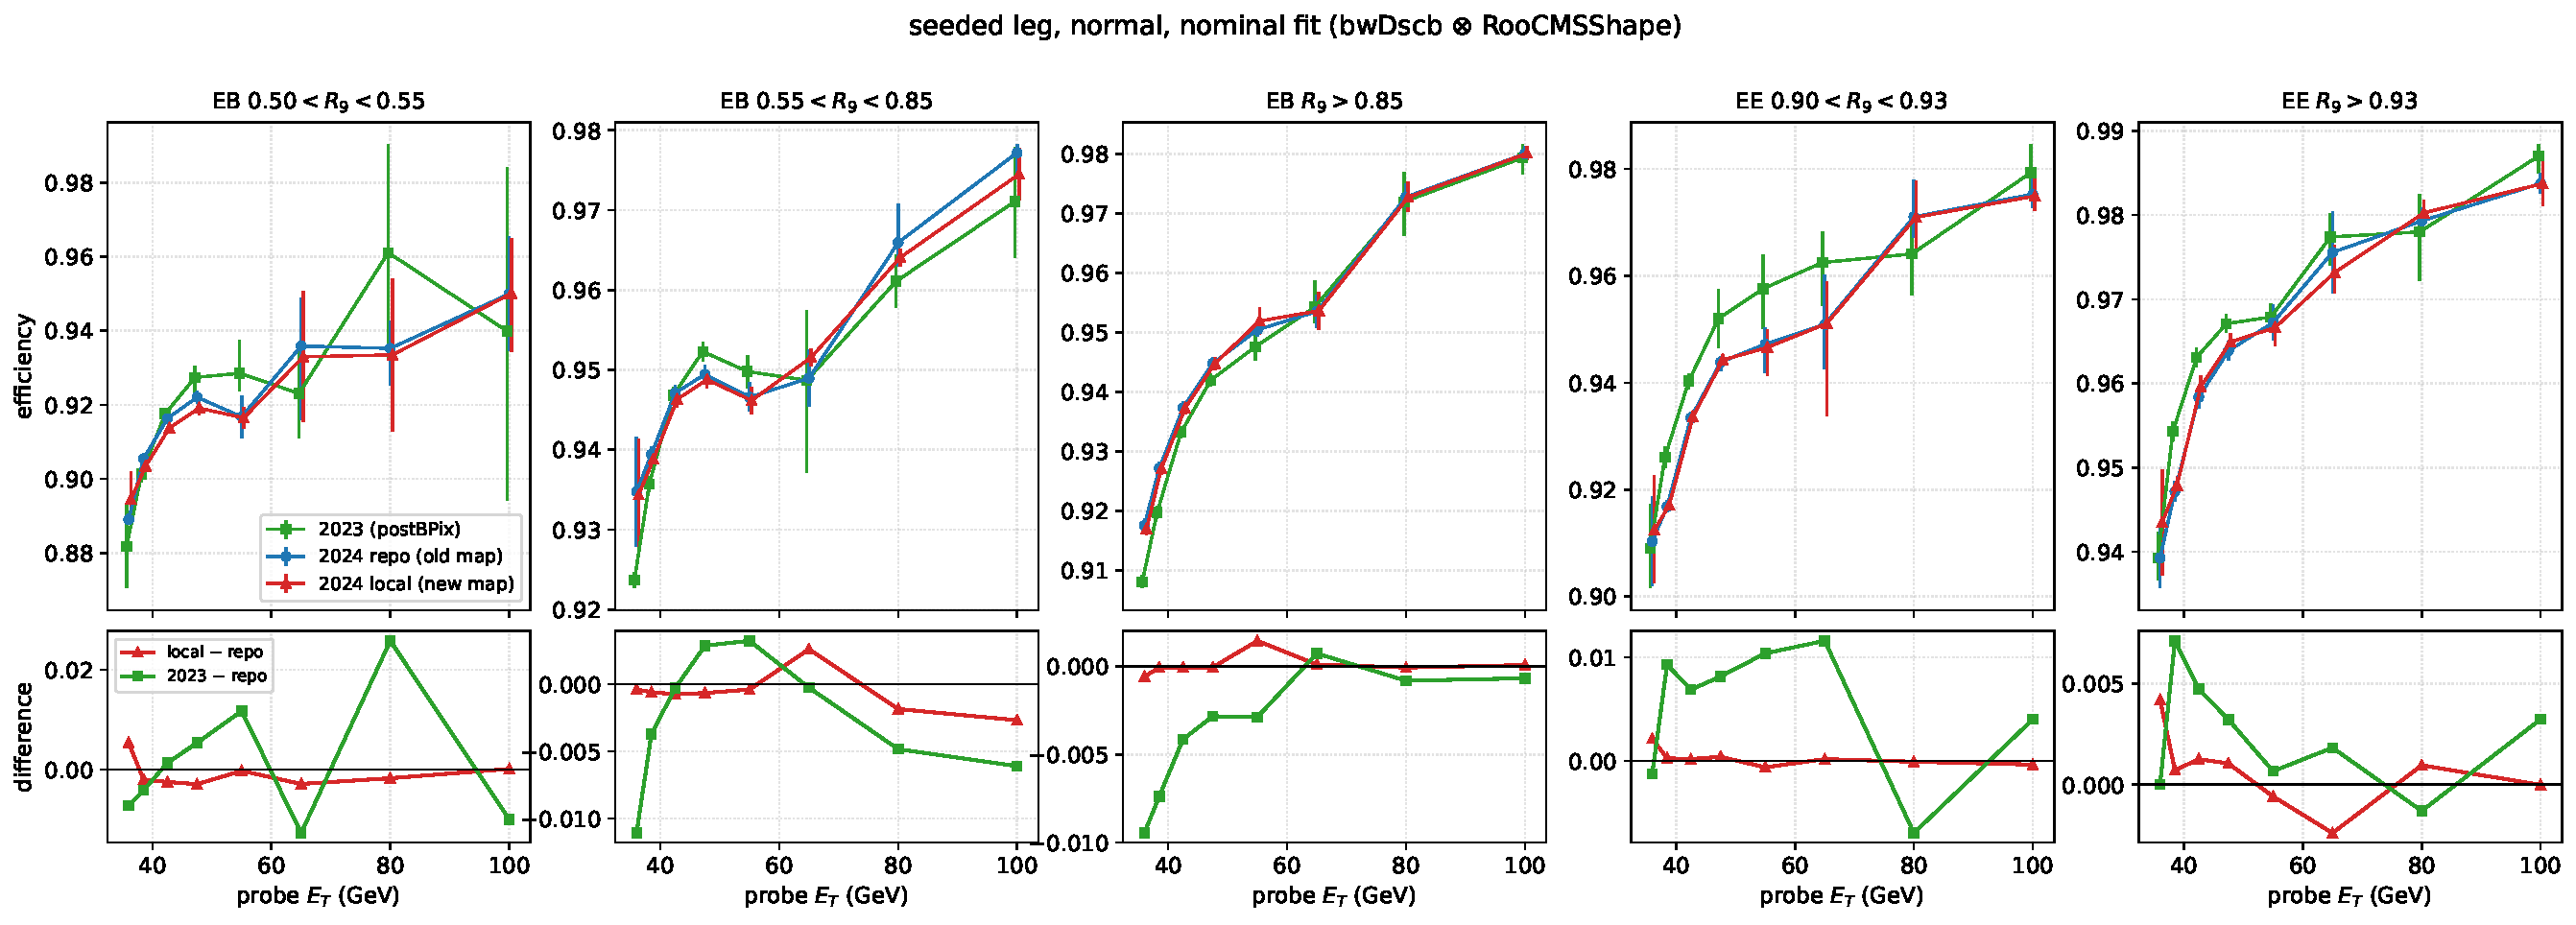
\includegraphics[width=0.98\linewidth,height=0.38\textheight,keepaspectratio]{eff/overview_normal_seed.pdf}}\\[2pt]
  \colorbox{white}{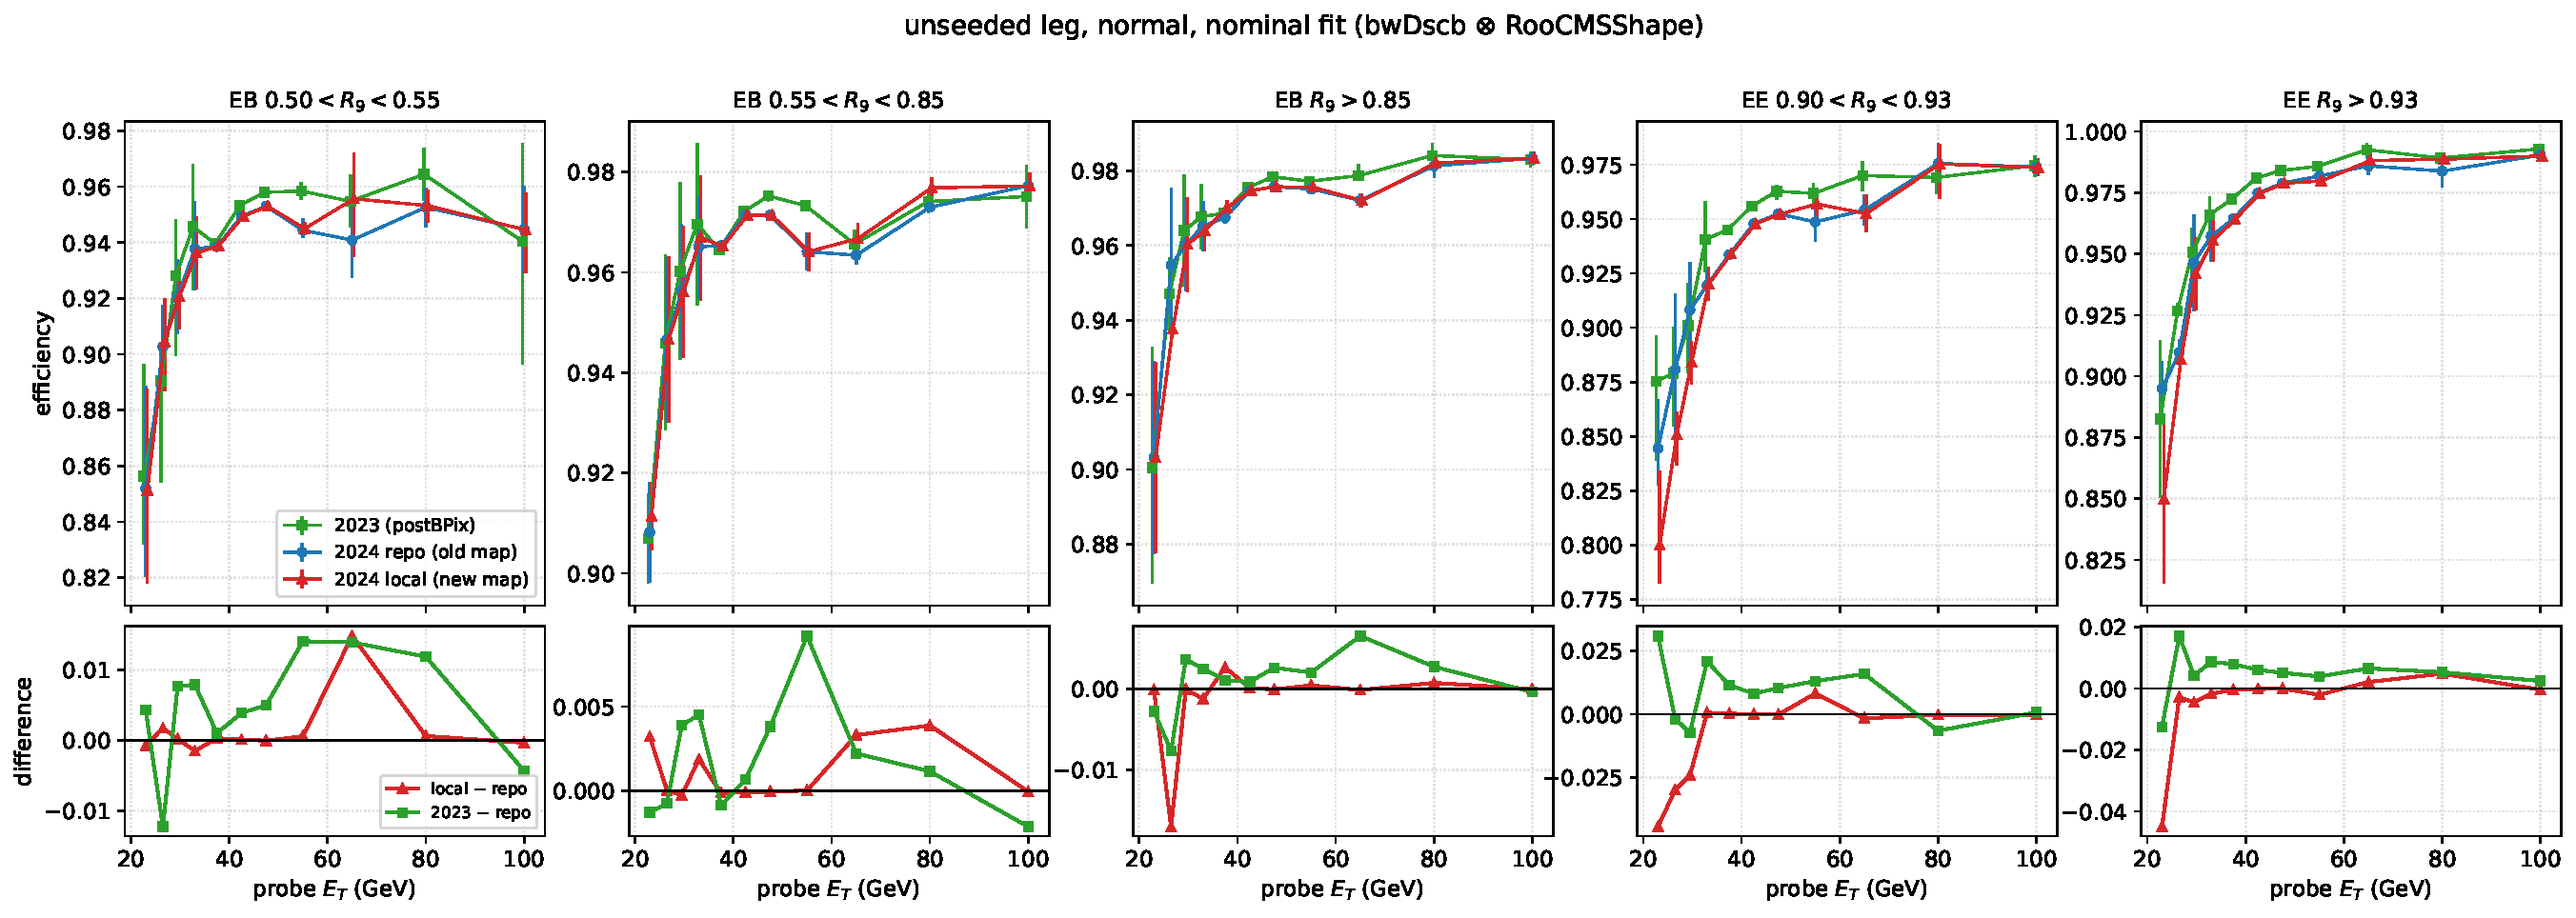
\includegraphics[width=0.98\linewidth,height=0.38\textheight,keepaspectratio]{eff/overview_normal_unseed.pdf}}
\end{frame}

\begin{frame}{Backup: fitted vs counting shift --- seeded, and fullPath}
  \centering
  \wimg{0.98\linewidth}{why/fit_vs_count_vs_pt_normal_seed.pdf}\\[2pt]
  \wimg{0.98\linewidth}{why/fit_vs_count_vs_pt_fullPath_unseed.pdf}\\[2pt]
  {\tiny\color{lightgrey} Top: seeded, normal. Bottom: unseeded, fullPath.}
\end{frame}

\begin{frame}{Backup: mean weight of passing vs failing probes --- seeded}
  \plotslide[0.98]{why/wpass_over_wfail_seed.pdf}{}
\end{frame}

\begin{frame}{Backup: fit pairs for shifts 2--4}
  \centering
  \colorbox{white}{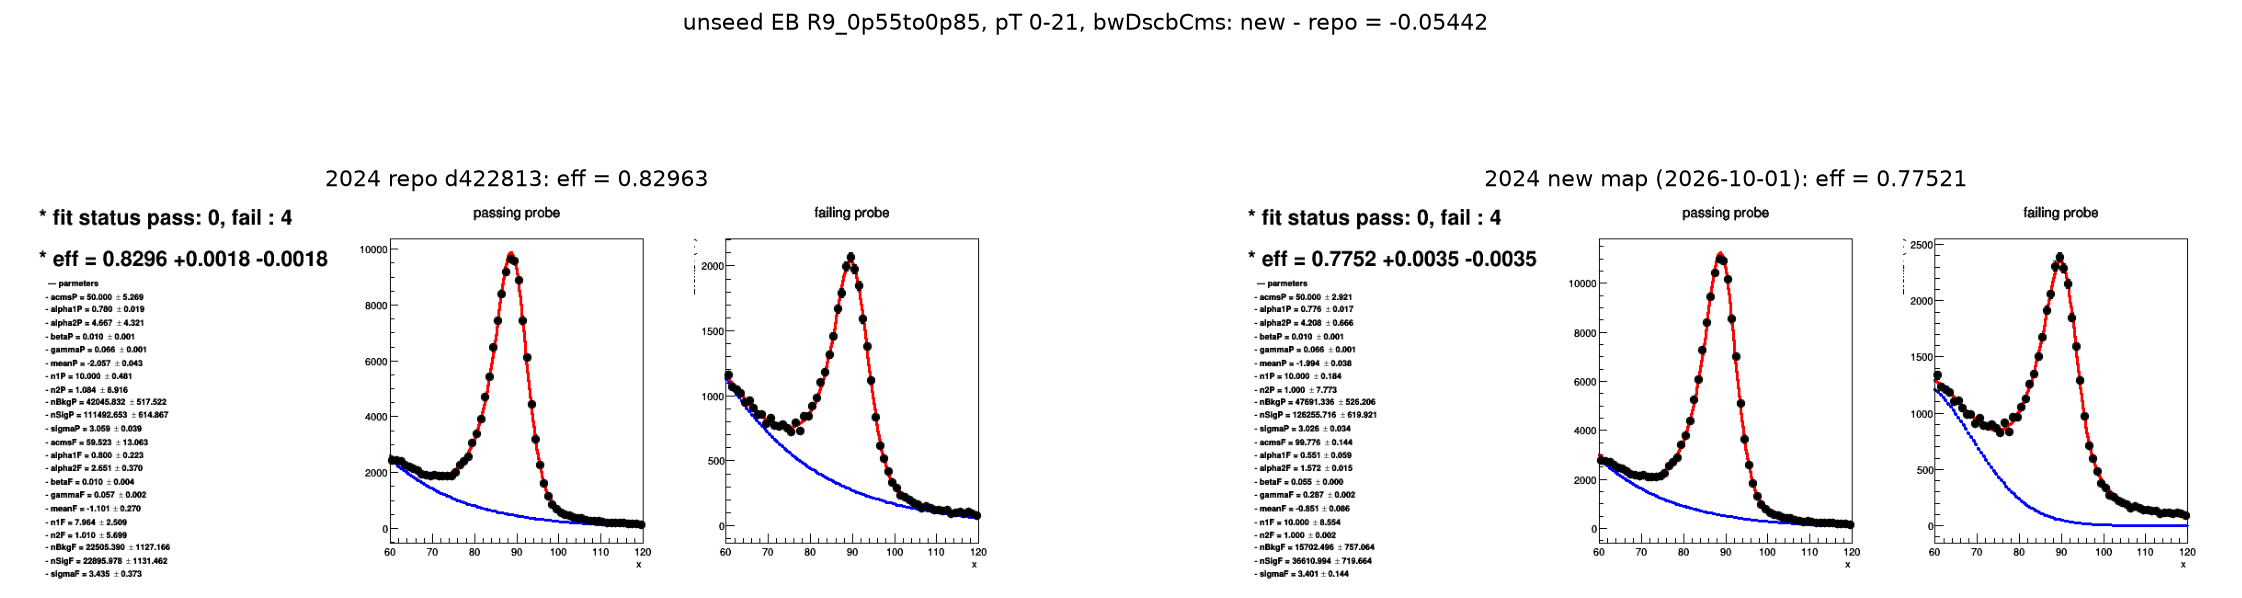
\includegraphics[width=0.85\linewidth,height=0.22\textheight,keepaspectratio]{why/fit_shift3_unseed_EB_R9_0p55to0p85_0_bwDscbCms.png}}\\[2pt]
  \colorbox{white}{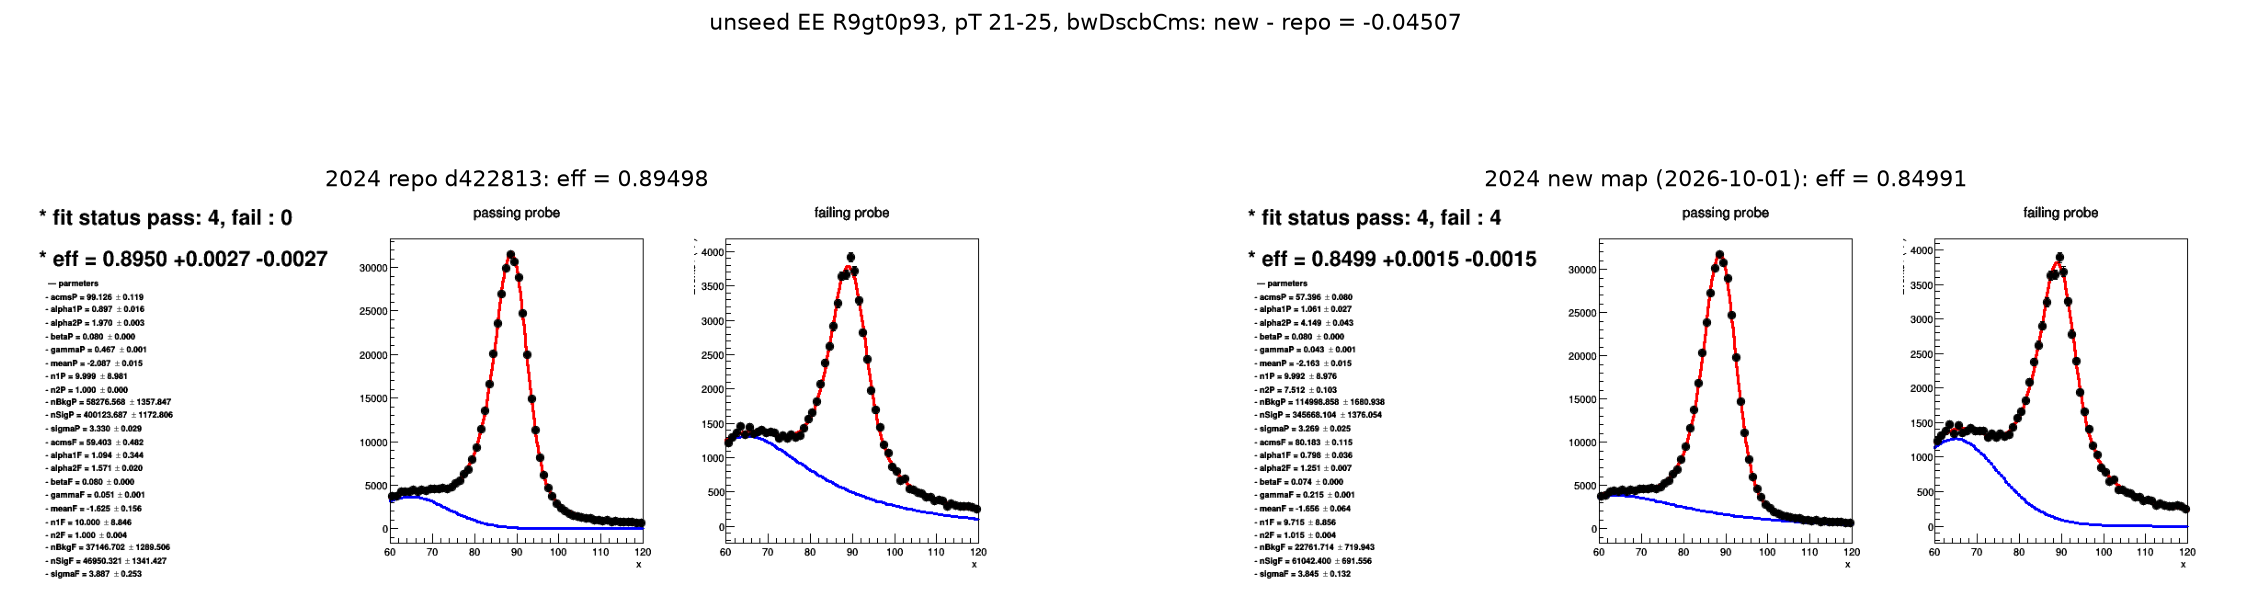
\includegraphics[width=0.85\linewidth,height=0.22\textheight,keepaspectratio]{why/fit_shift4_unseed_EE_R9gt0p93_21_bwDscbCms.png}}\\[2pt]
  \colorbox{white}{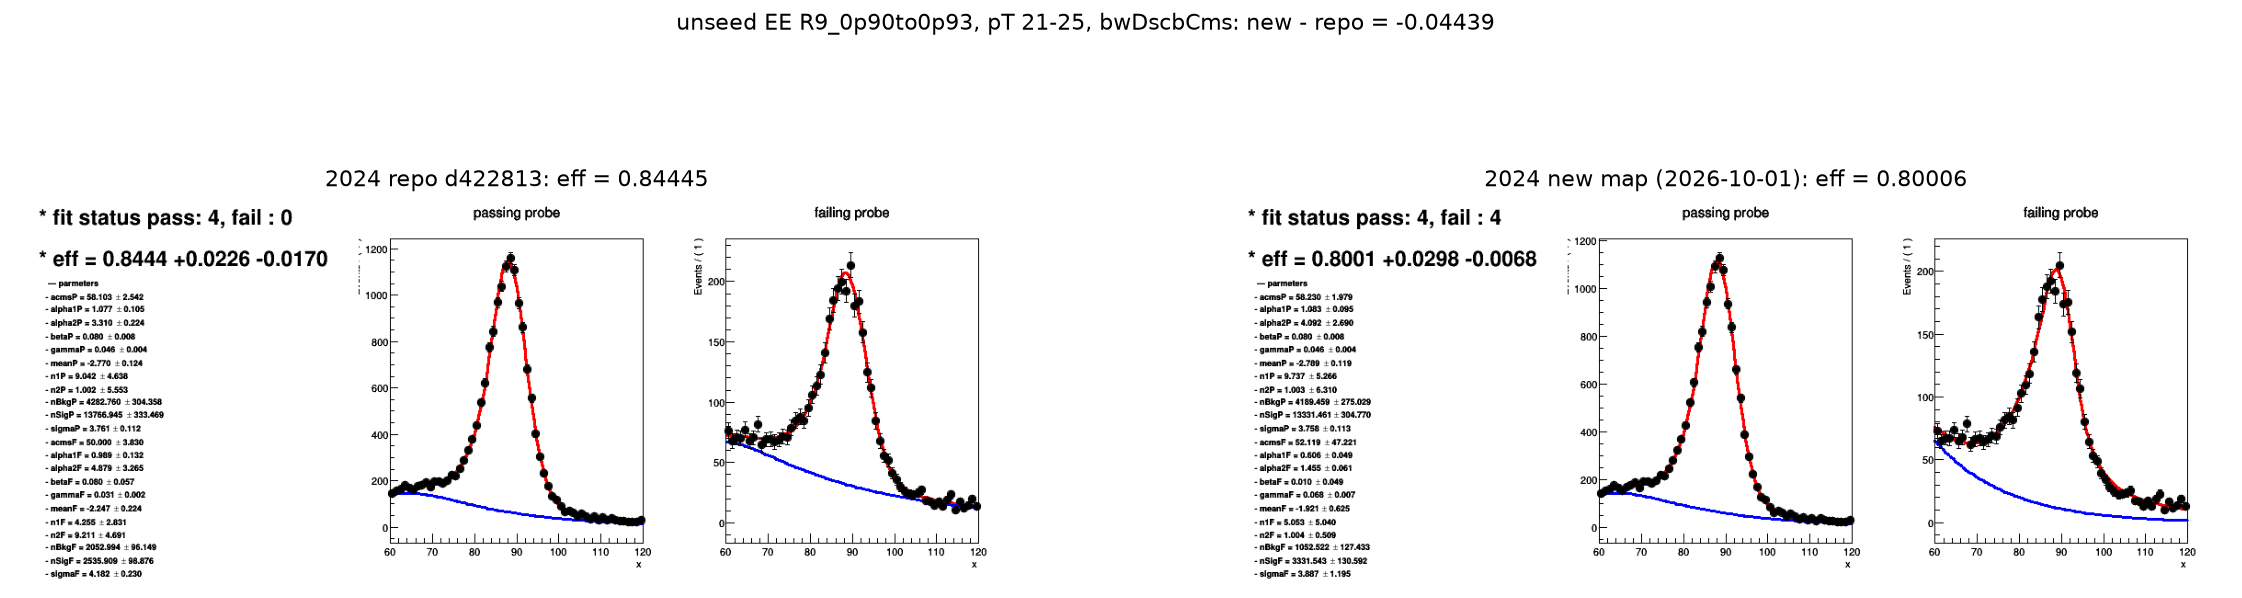
\includegraphics[width=0.85\linewidth,height=0.22\textheight,keepaspectratio]{why/fit_shift5_unseed_EE_R9_0p90to0p93_21_bwDscbCms.png}}\\[2pt]
  {\tiny\color{lightgrey} Left repo, right local. Unseeded EB $0.55<\RNine<0.85$ 0--21; EE $\RNine>0.93$ 21--25; EE $0.90<\RNine<0.93$ 21--25 (nominal fit).}
\end{frame}

\end{document}
